%%%%%%%%%%%%%%%%%%%%%%%%%%%%%%%%%%%%%%%%%%%%%%%%%%%%
% This will help you in writing your homebook
% Remember that the character % is a comment in latex
%
% chapter 1
\chapter{Introduction}
\label{Introduction}

%%%%%%%%%%%%%%%%%%%%%%%%%%%%%%%%%%%%%%%%%%%%%%%%%%%%%%%%%%%
% you can organize a chapter using sections -> \section{Simulating an inverter}
% or subsections -> \subsection{simulating a particular type of inverter}

%%%%%%   First section
    \indent In this short section the main concepts of the architecture are explained along with the related components.
    Additionaly, the added features which make up the Pro version of the DLX will be introduced along with related conceptual diagrams and schematics. 
    Lastly, the chapter will conclude with a mention on how the rest of the documentation is organized. 

\section{DLX Overview}
    The DLX we implemented consists in the computation and propagation of 32 bit instructions. 
    At a given time instant, multiple instructions of a partyicular assembly program are processed as this processor is constructed with a pipeline methodology.
    In particular, the stages of the pipeline for each instruction are given below:
    \begin{enumerate}
        \item Instruction Fetch;
        \item Instruction Decode;
        \item Execution;
        \item Memory;
        \item Write Back;
        \end{enumerate}
	\indent FUrthermore, there are three fundamental block of the implemented DLX which are involved during the pipelined execution of the program:
	\begin{enumerate}
        \item Datapath Unit;
        \item Control Unit;
        \item Hazard Unit;
        \end{enumerate}
		These components are explained in the following subsections of this chapter.
	\subsection{ The Datapath Unit }
    \indent The inclusion of the pipeline serves to increase the throughput of the overall program serving to reduce idle times of the processor. 
    The pipeline mechanism is noted most clearly in the datapath and control unit which are the fundamental hierierchical components of the processor.
    In Figure 2.1 the datapath with a pipelined mechanism is depicted. The figure also shows also some input signals which are entering the datapath. 
	These are control signals which come from another component called the Control Unit which sends appropriate control bits to the datapath depending on the instruction to be executed.
	Another important note about Figure 2.1 is that it depicts 2 memories, the instruction memory (IRAM) and the data memory (DRAM). These two memories
	are external components to the datapath and only interface it. Respectively, they serve an important role in the instruction fetch phase and memory phase of the instructions described later on.
    \begin{figure}[h!]
        \centering
        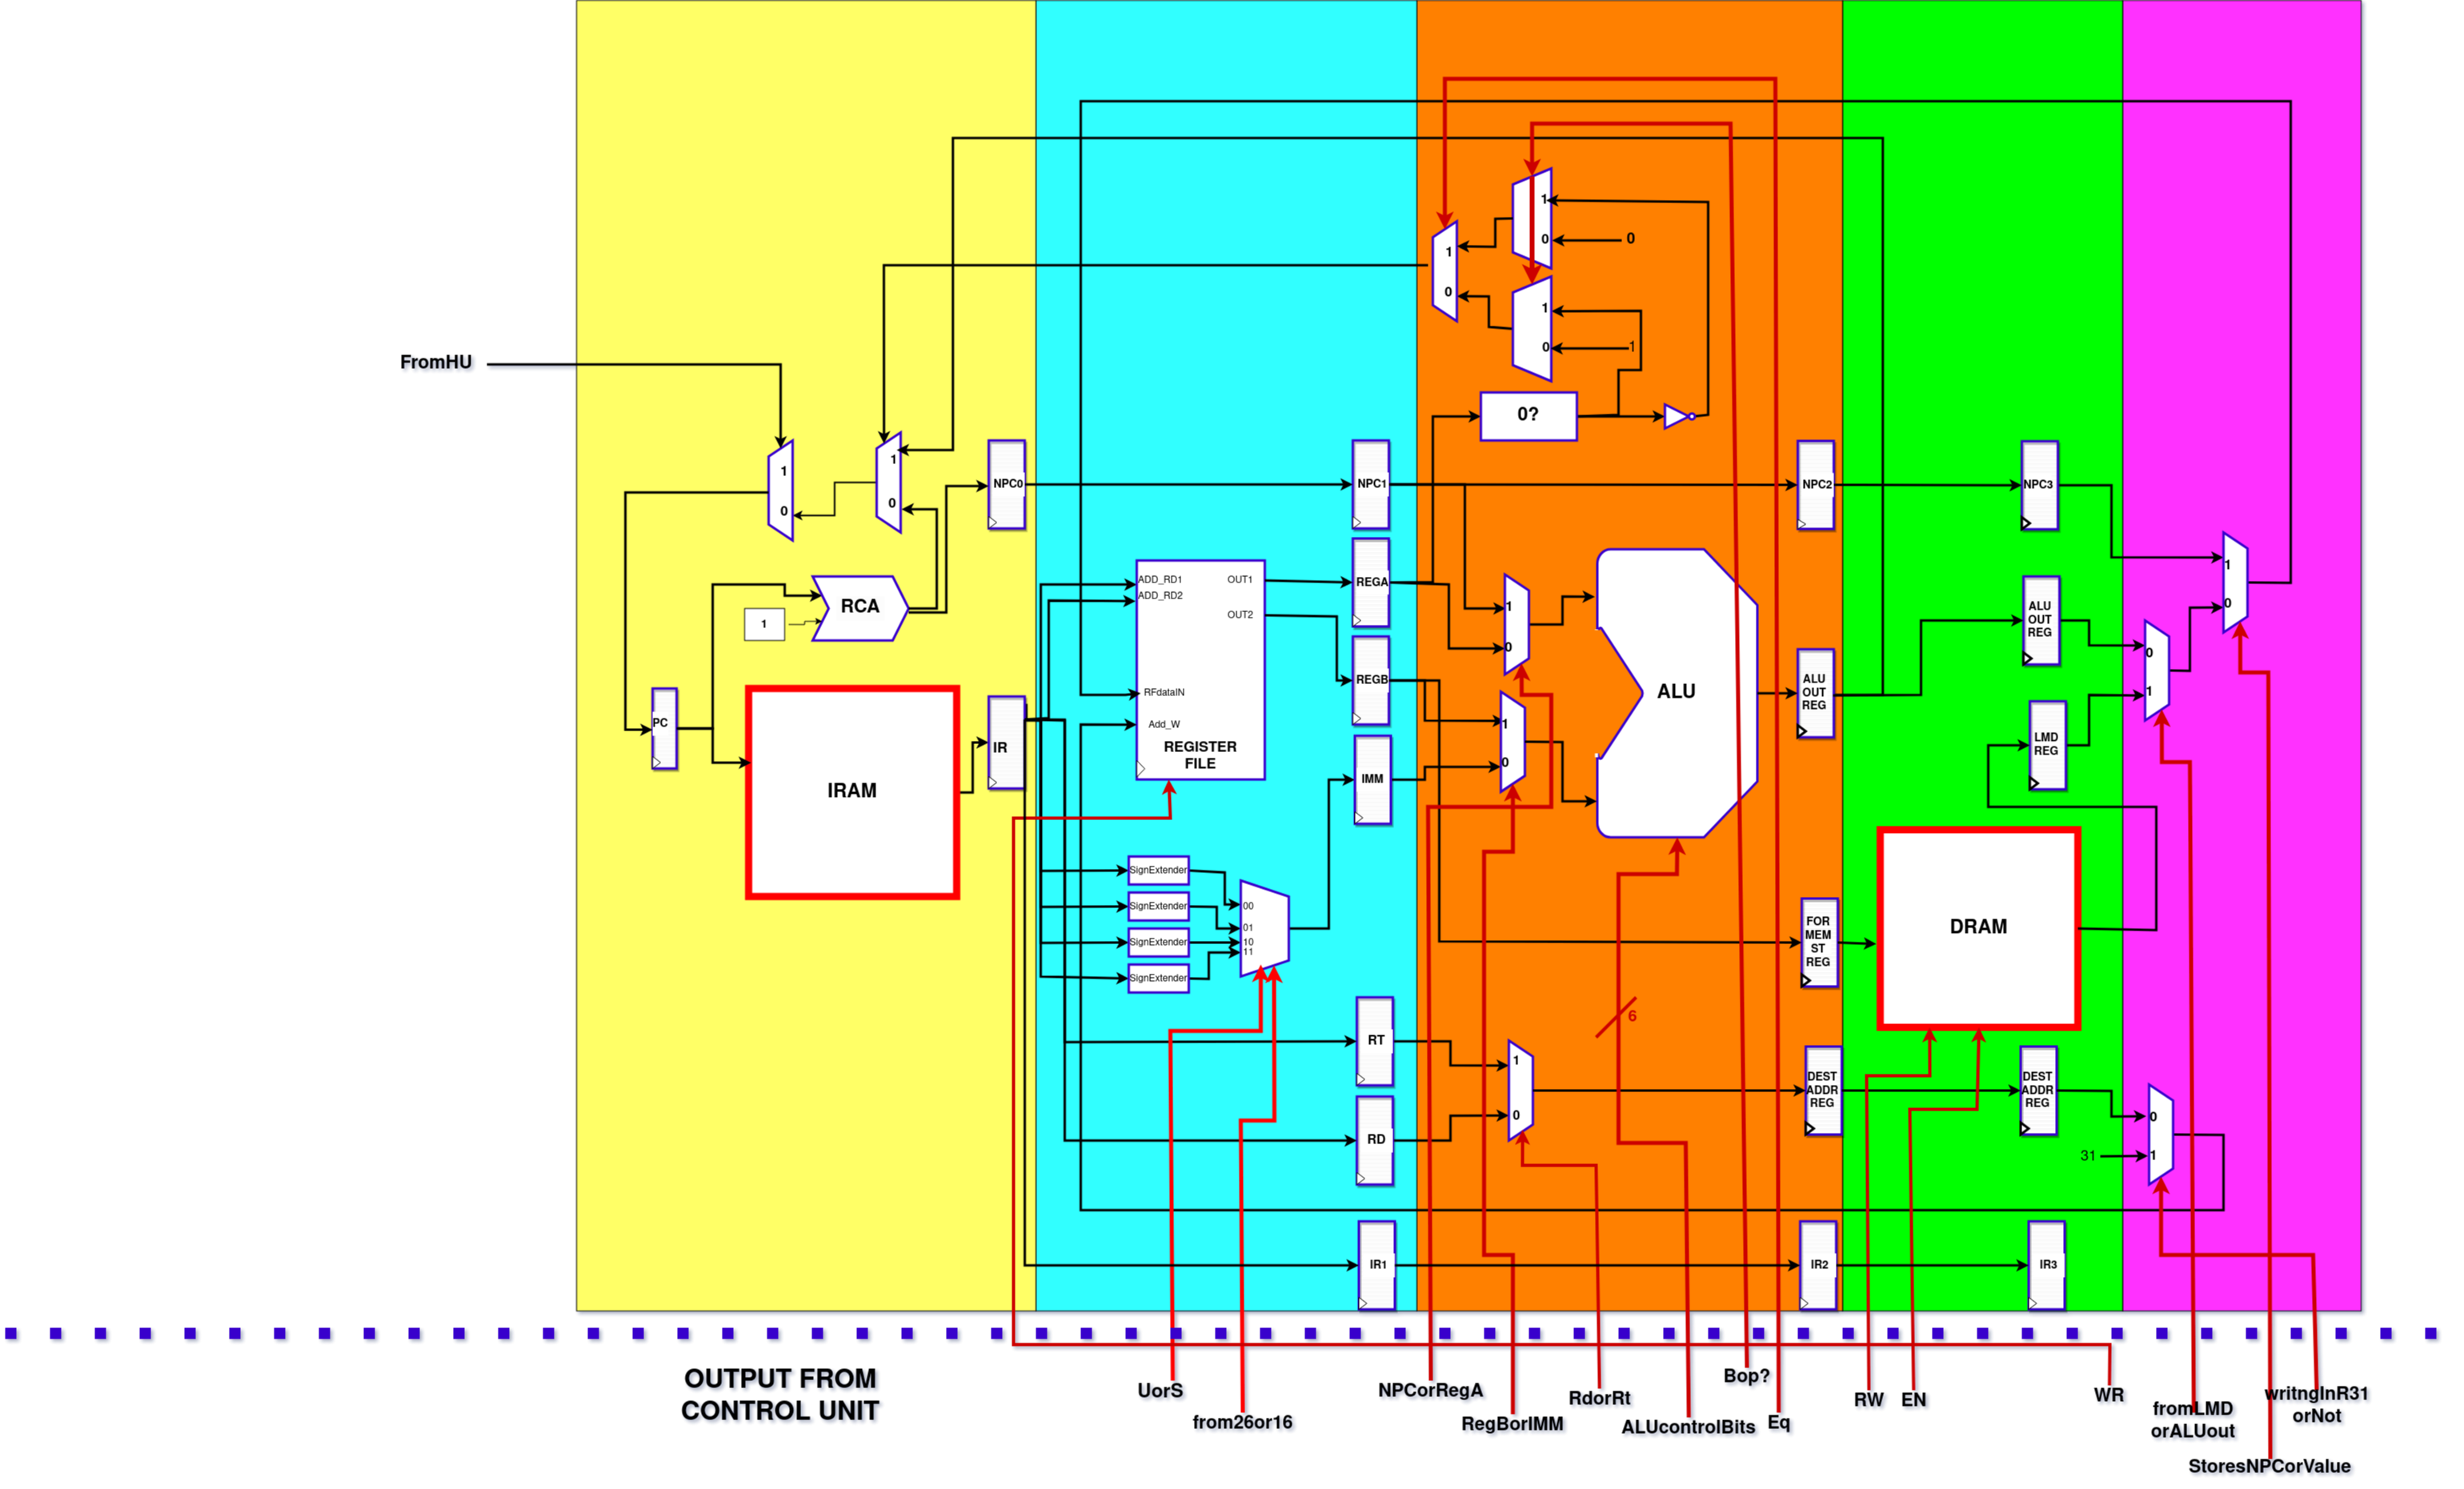
\includegraphics[scale = 0.15]
		{chapters/figures/DLXdatapath}
        \caption{DLX datapath component}
        \label{fig:datapathPic}
        \end{figure}

	\subsection{ The Control Unit and Hazard Unit }
	The Control Unit and hazard unit are side components which serve to control. Moreover, the control unit is constructed to give orders to the
	datapath about which instructions need to be executed but it gives such orders alertive to possible hazards which could be detected by the Hazard Unit. They will be discussed in a following chapter of the document.

	\section{Pro Version Features}
		The presented DLX has the following capabilities:
		\begin{enumerate}
			\item Extended Instruction set Architecture;
			\item Advanced Arithmetic Logic Unit;
			\item Extra component, the hazard unit;
			\end{enumerate}

			\newpage
		\subsection{ Extended Instruction set Architecture}
		The processor is able to run 50 instructions all listed in this section:
		\begin{enumerate}
			\item \textbf{RTYPE instructions}: ADD, SUB, AND, OR, SGE, SLE, SEQ, SNE, SRL, SRA, SLL, XOR, SLT, SGT, XNOR, NAND, NOR, ADDU, SUBU, SGEU, SGTU
			\item \textbf{ITYPE instructions}: NOP, ADDI, SUBI, ANDI, ORI, BEQZ, BNEZ, LDW, STW, XORI, SGEI, SLEI, SLLI, SNEI, SRLI, SEQI, SRAI, SLTI, SGTI, ADDUI,
			SUBUI, XNORI, NORI, NANDI, SGEUI, SGTUI, JR
			\item \textbf{JTYPE instructions}: JMP, JAL
			\end{enumerate}
		The datapath, control unit and hazard unit are able to process additional instructions with respect to the basic set of instructions.
		some of the additional instructions involve the ability to distinguish signed operands with unsigned for some operations, extra logical functionalities, more compare functionalities, and the ability
		to jump to an address stored in a particular register.

		\subsection{ Advanced Arithmetic Logic Unit }

		The inner components of the arithmetic Logic Unitc Unit are of advanced type. it is composed of a pentium 4 Carry LookAhead Spare Tree for more efficient addition and subtraction operations. 
		In addition, the logicals have been designed d with the T2 Logic methodology. The relevant schematics of the introduced inner components of the arithmetic logic unit are analyzed in Execution Unit section of the report

		\subsection{ Extra component, the hazard unit }

		This additional component is inside the DLX and it is able to make the distinguishment of the following type of hazards:

		\begin{enumerate}
			\item Read After Write Hazards 
			\item Control Hazard for branch instructions
			\item Jump detection
			\end{enumerate}

		These hazards will be detected and given to the control unit which will actuate the stall for the datapath. More information on the hazard unit will be given later on in the report.

		\section { Structure of the report }

		The structure of this documentation consists in the thorough analysis of the components in the datapath based on the pipeline stages. 
		Consequently an analysis on the implemented Control Unit and Hazard Unit is exposed explaining also their exhange of informatio.
		Lastly, an insight on the synthesis and physical design process is made available. In the next section we analyze the datapath starting from the components
		dedicated to the Fetch Unit.

